\section{Достаточные геометрические условия непрерывного
глобального покрытия}
\label{sec:geometric_conditions}

Для обеспечения глобального покрытия необходимо выполнение трех групп
условий, учитывающих геометрию взаимного расположения плоскостей.
Они включают коорбитальные, ретроградные и полярные условия. Следует
отметить, что представленные условия являются достаточными для
сферической модели Земли. Учитывая, что эллипсоид Земли вписан в данную
сферу (из-за сжатия у полюсов), выполнение представленных неравенств
гарантирует полное покрытие и для реальной эллипсоидальной модели.

\subsection{Условия на коорбитальные плоскости}

Коорбитальными назовем такие соседние плоскости орбит, в которых КА
движутся в одном направлении. Для предотвращения разрыва покрытия
между этими плоскостями необходимо, чтобы расстояние между ними не
превышало максимально допустимую величину \(D\). Геометрически это
расстояние определяется как сумма половины полосы покрытия одной
плоскости и радиуса зоны обзора соседней:
\begin{equation}
    D = \lambda_{\text{street}} + \theta.
\end{equation}

На основе векторов нормалей к плоскостям орбит, угловое расстояние между
двумя коорбитальными плоскостями \(i_{rel}\) через параметры наклонения и
разности ДВУ выражается как:
\begin{equation}
    \cos i_{rel} = \cos^2 i + \cos(\Delta\Omega) \sin^2 i.
\end{equation}
Приравнивая полученное расстояние к максимально допустимому
(\(i_{rel} = D\)), получаем ограничение на максимальную разницу ДВУ для
коорбитальных плоскостей:
\begin{equation}\label{eq:delta_omega_max}
    \Delta\Omega_{\text{max}} = \arccos\left(\frac{\cos D - \cos^2 i}{\sin^2 i}\right).
\end{equation}
Выбор \(\Delta\Omega \leq \Delta\Omega_{\text{max}}\) обеспечивает отсутствие
разрывов между соседними плоскостями при сонаправленном движении КА.


\begin{figure}[ht]
    \centering
    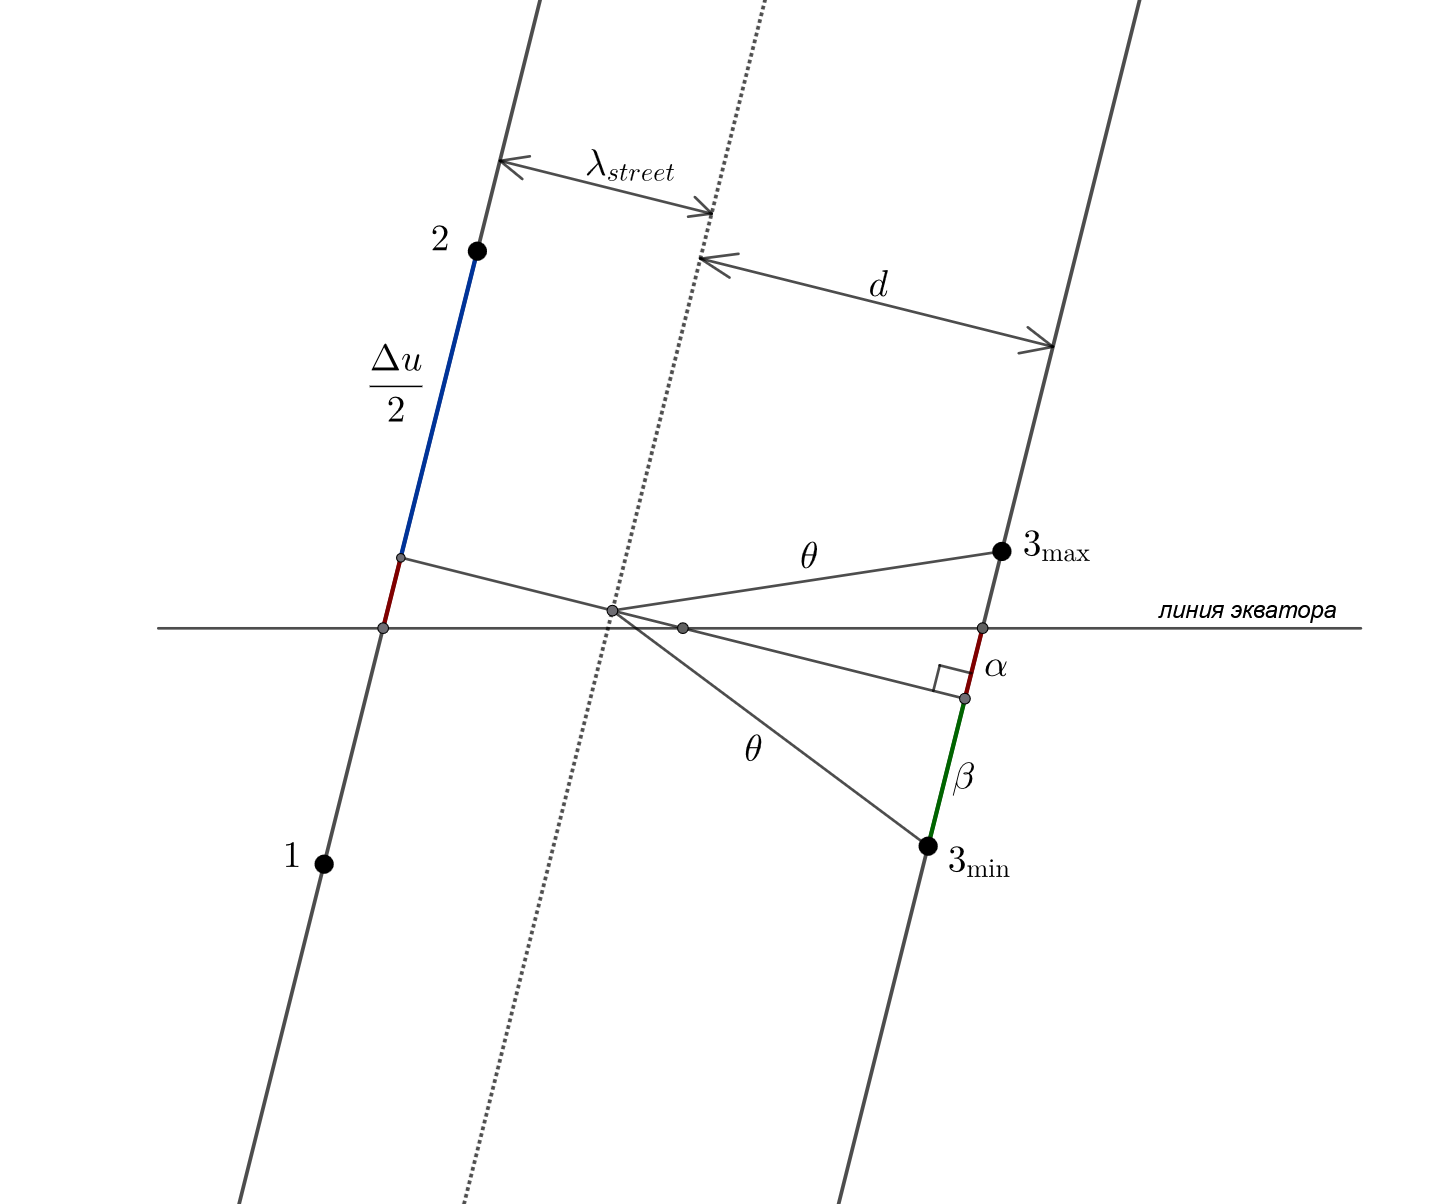
\includegraphics[width=0.75\textwidth]{pictures/phase_shift.png}
    \caption{Схема фазового сдвига между соседними плоскостями орбит}
    \label{fig:phase_shift}
\end{figure}

Также для коорбитальных плоскостей следует учитывать влияние фазового
сдвига \(f\). Он определяет относительное смещение трасс вдоль стыка двух
соседних плоскостей и, следовательно, влияет на то, как будут
перекрываться полосы покрытия. На рис.~\ref{fig:phase_shift} показана
схема взаимного расположения орбит при фазовом сдвиге. Рассмотрены две
соседние коорбитальные плоскости с разницей долгот восходящих узлов
$\Delta\Omega$. Будем считать, что выбранная $\Delta\Omega$ принадлежит
допустимому диапазону ДВУ. Угловое расстояние между этими плоскостями
обозначим $i_{rel}$.

Поскольку ширина полосы покрытия одной орбиты равна
$\lambda_{\text{street}}$, угловое расстояние от внешней границы полосы
покрытия одной орбиты до соседней на дуге $i_{rel}$ составит:
\begin{equation}
    d = i_{rel} - \lambda_{\text{street}}.
\end{equation}

Для того чтобы не произошло разрыва покрытия, КА на соседней орбите должен
находиться достаточно близко к границе полосы покрытия первой орбиты.
Геометрически это условие означает, что угловое расстояние между КА на
соседней орбите и границей полосы не должно превышать центральный угол зоны
обзора $\theta$.

На орбите слева от пересечения дуги $i_{rel}$ вниз на $\Delta u/2$ находится
первый КА, вверх на $\Delta u/2$ находится второй КА. Обозначим допустимый
диапазон аргумента широты КА на соседней орбите как $u_{3,\min}$ и
$u_{3,\max}$.

Отсчитываем фазовый сдвиг от первого КА на левой орбите вверх по
направлению движения КА. Если $u_3$ принадлежит диапазону
$[u_{3,\min}, u_{3,\max}]$, то разрывов в покрытии между соседними
плоскостями происходить не будет. Выразим тогда допустимые сдвиги фаз:
\begin{equation}\label{eq:phase_shift}
    f_{max} = \frac{\Delta u}{2} + \beta - 2\alpha
\end{equation}
\begin{equation}
    f_{min} = \frac{\Delta u}{2} - \beta - 2\alpha
\end{equation}

Из сферической геометрии можем выразить допустимое отклонение по
аргументу широты $\beta$ и смещение $\alpha$.
\begin{equation}
    \beta = \arccos \left(  \frac{\cos \theta}{\cos d} \right)
\end{equation}

\begin{equation}
    \alpha = \arccos \left( \frac{\cos(\frac{\Delta\Omega}{2})}{\cos(\frac{i_{rel}}{2})} \right)
\end{equation}


Подставляя выражения для \(\alpha\) и \(\beta\) в \eqref{eq:phase_shift}, 
получаем итоговые аналитические формулы для расчета границ фазового сдвига:
\begin{equation}
    f_{max} = \frac{\Delta u}{2} + \arccos \left( \frac{\cos \theta}{\cos d} \right)
    - 2 \arccos \left( \frac{\cos\left(\frac{\Delta\Omega}{2}\right)}{\cos\left(
        \frac{i_{rel}}{2}\right)} \right)
\end{equation}
\begin{equation}
    f_{min} = \frac{\Delta u}{2} - \arccos \left( \frac{\cos \theta}{\cos d} \right)
    - 2 \arccos \left( \frac{\cos\left(\frac{\Delta\Omega}{2}\right)}{\cos\left(
        \frac{i_{rel}}{2}\right)} \right)
\end{equation}

Выбор фазового сдвига \(f \in [f_{\min}, f_{\max}]\) гарантирует
непрерывность покрытия на стыках коорбитальных плоскостей. Таким образом,
при соблюдении указанных ограничений разрывы покрытия между соседними
коорбитальными плоскостями не возникают.


\subsection{Условия на ретроградные плоскости}

Ретроградными называются соседние плоскости, в которых КА
движутся в противоположных направлениях. В
Walker-построении такими плоскостями являются первая и последняя.

При заданном числе плоскостей \(P\) долгота восходящего узла последней
плоскости определяется как
\begin{equation}
    \Omega_P = (P-1)\Delta\Omega_{\text{max}},
\end{equation}
где \(\Delta\Omega_{\text{max}}\) — максимальное значение шага по долготе
восходящего узла, полученное для коорбитальных плоскостей (\ref{eq:delta_omega_max}).

Если \(\Delta\Omega_{\text{max}} < \pi\), то требуется проверить, не
будет ли разрыва в покрытии на ретроградных орбитах.

Для ретроградных плоскостей максимальное допустимое угловое расстояние
между ними определяется как сумма двух полос покрытия:
\begin{equation}
    D_{re} = 2\lambda_{\text{street}}.
\end{equation}

Угловое расстояние между первой и последней плоскостью можно вычислить
следующим образом:
\begin{equation}
    \cos i_{rel} = \cos^2 i + \cos\bigl((P-1)\Delta\Omega_{\text{max}}\bigr)\sin^2 i.
\end{equation}
Это расстояние \(i_{rel}\) соответствует углу между плоскостями, если оно
рассматривается между их восходящими узлами.

Для оценки разрыва покрытия между ретроградными плоскостями требуется
получить угол, измеряемый именно между ретроградными плоскостями. Он равен:
\begin{equation}
    i_{rel}^{(re)} = \pi - i_{rel}.
\end{equation}
Если выполняется условие \(i_{rel}^{(re)} \leq D_{re}\),
то покрытие на ретроградных плоскостях остается непрерывным. В противном
случае возникает разрыв.

В отличие от коорбитального случая, фазовый сдвиг \(f\) не оказывает
влияния на покрытие на ретроградных орбитах. Они движутся навстречу друг
другу, и их геометрическое взаимное расположение жестко фиксировано в
любой момент времени.

Приравнивая угловое расстояние между первой и последней плоскостями
\(i_{rel}^{(re)}\) к \(D_{re}\), получаем выражение для минимально
допустимой разницы ДВУ, при которой не возникает разрыва в покрытии:
\begin{equation}
    \Delta\Omega_{\text{min}} = \frac{1}{(P-1)} \arccos\left(
        \frac{-\cos D_{re} - \cos^2 i}{\sin^2 i}\right).
\end{equation}

Таким образом, для ретроградных плоскостей разница ДВУ выбирается исходя
из условия \(\Delta\Omega \geq \Delta\Omega_{\text{min}}\). При этом
геометрическое положение таких плоскостей остается фиксированным во время
движения спутников, и фазовый сдвиг не влияет на непрерывность покрытия.
